\documentclass[
 reprint,
 amsmath,amssymb,
 aps,
]{revtex4-1}

\usepackage{graphicx}  
\usepackage{epstopdf}
\usepackage{dcolumn}
\usepackage{bm}	
\usepackage{amsmath}			
\usepackage{amsfonts}			
\usepackage{amssymb}			
\usepackage{latexsym}		
\usepackage{color}
\usepackage{ stmaryrd }

\def\tc{\textcolor{red}}
\begin{document}
\title{ Influence of spectral dispersion and polarization smoothing on the  growth of the forward Brillouin scatter}
\author{C. Ruyer}\email{charles.ruyer@cea.fr}
\affiliation{CEA, DAM, DIF, F-91297 Arpajon, France}
%\author{M. Grech}
%\affiliation{LULI - CNRS, CEA, UPMC Univ Paris 06: Sorbonne Universit\'e, Ecole Polytechnique, Institut Polytechnique de Paris - F-91128 Palaiseau Cedex, France}
\author{A. Debayle}
\affiliation{CEA, DAM, DIF, F-91297 Arpajon, France}
\author{P. Loiseau}
\affiliation{CEA, DAM, DIF, F-91297 Arpajon, France}
%\author{M. Casanova}
%\affiliation{CEA, DAM, DIF, F-91297 Arpajon, France}
\author{P. E. Masson-Laborde}
\affiliation{CEA, DAM, DIF, F-91297 Arpajon, France}

\begin{abstract} 
The forward Brillouin scattering of a realistic laser is studied by mean of analytical dispersion relations, focusing on the role of temporal smoothing on the spatial growth. Both   longitudinal and transverse  spectral dispersion are addressed and analysed  for  typical ICF plasma conditions,  demonstrating that 
the scatter growth is hardly affected and suggesting that a beam aperture increase can   be expected during the propagation LMJ, NIF or SG-III-class laser pulses resulting from the forward Brillouin scattering.  Hydrodynamic paraxial HERA simulations confirm our predictions.
\end{abstract}

\maketitle

\section{Introduction}
Unprecedented energy levels may be reached when matter is irradiated with a LMJ, NIF or SG-III-class laser pulses \cite{Cavailler_2005,Lindl_2004,MRE_Zheng_2017}, allowing to probe matter under extreme conditions of interest for astrophysical studies, ignition purposes or high energy density physics \cite[]{Drake2006}.
During these experiments, the laser heat source invariably ends up propagating through a plasma, brought  into existence by  an exploded foil,  the ionisation of a gaz or from both. 
The coupling of the light beam with the plasma animates numerous wave mixing processes that leads to abnormal plasma heating \cite[]{PRL_Schurtz_2009}, fast particle generation \cite[]{POP_Rousseaux_2002,MRE_Tikhonchuk_2021},  significant backscattering  \cite[]{POP_MacGowan_1996,POP_Montgomery_1998,POP_Huller_2020}, beam pointing direction deviation \cite[]{PRL_Moody_96,PRL_Hinkel_1996} or   noteworthy modification of the pulse propagation and subsequent energy deposition  \cite[]{POP_Schmitt_Afeyan_98,POP_Grech_2006}.
Unfortunately, these processes are not independent from each other and, most of the time, they may occur concurrently, adding to the complexity of the laser plasma interaction accurate description. 
In order to improve the control on the pulse propagation, most high energy laser facility use spatial smoothing techniques such as Random Phase Plates (RPP)  and Spectral Dispersion (SSD) which results in degrading the spatial or temporal laser coherence, respectively \cite[]{Kato_1984,Skupski_1989}. 
The produced intensity profile is composed of microns-scale fluctuations, the so-called speckles or hot spots which may vanish and change position periodically  \cite[]{Garnier_1999,Garnier_2001,POP_Duluc_2019}.
Many experimental and theoretical studies demonstrate, that degrading the laser coherence indeed improves the laser propagation quality \cite[]{POP_Hinkel_1998,PRL_Myatt_2001,NatPhys_Glenzer,NatPhys_Labaune,PRL_Grech_2009}, regrettably, without completely stabilizing most wave mixing processes as notably, the backward Brillouin \cite[]{JRE_Moody_93,Berger_1995}, side  Raman scattering \cite[]{PRE_Michel_2019} or  cross beam energy transfer \cite[]{PRL_Michel_2009,Glenzer2010,PRL_Neuville_2016cbet,PTA_Huller_2020} have been characterized in these conditions (see also Ref. \cite[]{Kirkwood_2013}). 
Hence, the groundwork and predictions associated with these experiments is further complicated by the entanglement between the  laser plasma instabilities (LPI) and the pump wave controlled incoherence.

Important kinetic first principle simulations tools such as "particle-in-cell" codes  \cite[]{Lefebvre_2003,fonseca_osiris,Smilei}  allow  to address most LPI all at once, at the expense of a formidable numerical cost that restrains the simulations to a very small domains. For addressing  larger and longer systems,  hydrodynamic-based simulation codes coupled with an often approximated Maxwell solver are of great usefulness \cite{Berger_1995,Still_2006,Loiseau_2006, Huller_2006}, even though they fail to capture important mechanisms  such as non-local thermal diffusion \cite[]{POP_Schurtz_2000,PRL_Froula_2007},
particle trapping   \cite[]{POP_Benisti_2008,POP_Berger_2013} or multi-ion species effects \cite[]{POP_Williams_95,Abramowitz,POP_Berger_2005b,Ruyer_2020}.
In this publication, we will concentrate on another tool,  as important as the two previous examples, and which may help understand and predict the wave mixing processes at stake and their condition of occurrence. The analytical dispersion relations derived in Ref.  \cite[]{Ruyer_FSBS} opens the way for accounting properly for the pump smoothing techniques on the growth of the backward/forward Brillouin or filamentation scatter. 
We will address in this study the particular case of the Forward Stimulated  Brillouin Scattering (FSBS), and generalize the results of Ref.  \cite[]{Ruyer_FSBS} to the case of temporally smoothed pump waves as used in most laser facilities. Two types of spectral dispersion will be investigated and compared and the impact of the SSD parameters on the propagation quality will be analyzed. 
As the exact modeling of SSD in the scatter wave dispersion relation involves extensive algebra, we will keep the plasma response to its most simple form not to add further complexity. We thus restrain this study to the fluid formalism of a single ion species plasma based on   Ref.  \cite[]{Ruyer_FSBS}  which indicates that, in this case, kinetic effects are negligible regarding the scattering of  RPP beams.
Hence, a comparison with hydrodynamic HERA simulations with a paraxial description of the  laser pulse will be carried.
We will also briefly address the combination of SSD with Polarization Smoothing (PS),
before concluding on our results.

Throughout this publication, the SI unit system will be used while dropping the Boltzmann constant and noting the vectors in bold symbols.


\section{Accounting for the spatial smoothing and spectral dispersion of the pump on the forward scatter growth}

\subsection{Fluid plasma response}
The dispersion relations of the stimulated forward Brillouin scattering (FSBS) and beam filamentation ensue from the combination of the linearized propagation of the laser beam described by  Maxwell equations with a linearized plasma response, either kinetic of fluid. 

Regarding the latter, we will settle with the description of Ref. \cite[]{Ruyer_FSBS} which shows that the linearized density fluctuations, $\delta n_e /n_{e0}$ may be related to the  perturbed scattered  amplitude $\delta E$ in the Fourier space $(\omega_s,\mathbf{k}_s)$ and the pump field  $E_p$.
Introducing $\epsilon_0$, $n_c$, $c_s$, $\nu=\vert\mathbf{k}_s\vert \gamma_0 c_s$, $n_{e0}$, $Z_s$, $A_s$, $T_{s}$, $m_s$ the permittivity of vacuum, laser critical density, sound speed, Landau acoustic damping rate, averaged electron density, charge number, mass number temperature and mass of the $s$-th species respectively, 

\begin{align}
   \frac{\delta n_e }{n_{e0}}(\omega_s,\mathbf{k}_s) = -\alpha_{f}(v_\phi) \frac{A_k\epsilon_0 E_p}{n_c T_e}\otimes   \delta E  \, ,\label{eq:fd} \\
%   \alpha_k  =\frac{\mathcal{Z}'( \zeta_e) }{2}\frac{\sum_i\mathcal{Z}'( \zeta_i)\frac{  Z_iT_e}{ T_i }\frac{  Z_in_i}{ n_e }   }{  \mathcal{Z}'( \zeta_e)+ \sum_i\mathcal{Z}'( \zeta_i)\frac{  Z_iT_e}{ T_i }\frac{ Z_i n_i}{ n_e }  }\, ,\label{eq:alphak} \\
   \alpha_f = \frac{Z_iT_e}{m_ic_s^2} \frac{ c_s^2}{ c_s^2-v_\phi^2 -2iv_\phi c_s \gamma_0}\, , \label{eq:alphaf}
\end{align}
with $v_\phi = \omega/\vert \mathbf{k}_s\vert$.
%\begin{align}
%\zeta_{e/i} = \frac{   \omega_s }{   \vert\mathbf{k}_s\vert }  \sqrt{ \frac{ m_{e/i } }{ 2T_{e/i }}  }  \label{eq:xi} \, , \\
%v_\phi =  \frac{   \omega_s }{   \vert\mathbf{k}_s\vert %}\, . \label{eq:vphi}
%\end{align}
We made use of %$\mathcal{Z}$, the plasma dispersion function \cite{Fried_Gell-Mann_1960} and of  
$A_k$, the  non-local thermal correction to the ponderomotive force  as introduced in Refs. \cite[]{POP_Kaiser_1993,Bychenkov_2000}, 
\begin{align}
     A_k(u)   &= \frac{1}{2} +Z\left( \frac{0.074}{u^2}+ \frac{0.88}{u^{4/7}} + \frac{2.54}{1+5.5u^2} \right) \, ,\nonumber \\ 
     u &=\vert \mathbf{k}_s \vert\lambda_\mathrm{mfp} \sqrt{Z_i}\label{eq:nl}\, ,
\end{align}
where $\lambda_\mathrm{mfp}$ is the  electron mean-free-path.

The kinetic collisionless linearized plasma response, is, at this stage,  straightforward to account for as it consists in replacing  $\alpha_f $ in Eq. \eqref{eq:fd} by its kinetic counterpart (see  Ref. \cite[]{Ruyer_FSBS}), although out of the scope of this manuscript. 
Moreover,   the plasma response to driven acoustic waves should include, in addition to the Landau damping, Coulomb collisions effects as derived from the Fokker Planck equation in Ref. \cite[]{POP_Berger_2005}. The  $\alpha_f $ factor in Eq. \eqref{eq:fd}  would be replaced by 
\begin{equation}
    \alpha_f^\mathrm{coll} = \frac{X_e(\omega,\mathbf{k}_s)}{2\epsilon(\omega,\mathbf{k}_s)} \, , \label{eq:alphafc}
\end{equation}
where $\epsilon$ and $X_e$ are given by Eqs. (29) and (30) of Ref. \cite[]{POP_Berger_2005}, respectively,  with thus use of Eqs. (31)-(40).
Note that the subsequent dispersion relation predictions will be confronted to an hydrodynamic code  which does not account for these Coulomb collisions effects. Hence Eqs. \eqref{eq:fd}-\eqref{eq:alphaf} will be used afterward \tc{with a collisional Landau damping rate as published in \cite[]{casanova_1989}}, and keeping in mind that in realistic conditions Eq. \eqref{eq:alphafc} is more appropriate. 

\subsection{Propagation of the RPP and  SSD pulse with and without polarisation smoothing}
The broadening of the  laser temporal spatial (RPP) and temporal (SSD) spectrum \cite{Kato_1984,Skupski_1989} is  routinely used in multi-kilojoule class laser facilities for improving the beam propagation quality \cite[]{NatPhys_Glenzer,NatPhys_Labaune,POP_Delamater_2000} and decreasing the amount of backscattering \cite[]{POP_Duluc_2019}. 
The associated electric field may be modeled, in a $D$-dimension system,  through \cite[]{POP_Rose_98,Rothenberg_97,Videau_1999}, 
\begin{align}
    &E_p(x,\mathbf{r}_\perp,t) =\frac{E_0}{N^{D-1}} \sum_{l=-m}^{+m}  e^{i k_l x }J_l(m) \sum_{\mathbf{n} }  
    %\exp\left[-i\omega_lt +i\omega_l T_{r} f_{T/L}[\mathbf{k}_\perp(\mathbf{n},l)] +i \mathbf{k}_\perp(\mathbf{n},l)\cdot \mathbf{r}_\perp +i\phi_{\mathbf{n}}  \right] 
    e^{i\Theta}
    \, , \label{eq:essd}  \\
   & \Theta = -\omega_lt +\omega_l T_{r} f_{T/L}[\mathbf{k}_\perp(\mathbf{n},l)] + \mathbf{k}_\perp(\mathbf{n},l)\cdot \mathbf{r}_\perp +\phi_{\mathbf{n}} \, ,\\
   & \omega_l= \omega_0+l \omega_m \\
   & k_l = k_0(1+l\omega_m/\omega_0 ) = \omega_l\eta /c \\
    &\mathbf{k}_{\perp }( \mathbf{n},l)= \mathbf{n}  2k_m(1+l\omega_m/\omega_0 )/N\, .\label{eq:kp}
\end{align}
We introduced $N$, $\eta$, $ w_m$, $m$ and $T_{r}$, the number of diffracting elements in the phase plate, the refraction index, the modulation frequency, the number of modes and the SSD delay, respectively as well as  $J_l(m)$, the Bessel function of the first kind.
The phases $\Phi_{\mathbf{n}}$ are independent random variables taking the values $0$ or $\pi$ with equal probability.
Under these conditions, and for $\langle w\rangle$ representing the statistical average of the random variable $w$,   we note   that,
 \begin{equation}\label{eq:d}
 \langle e^{i\Phi_{\mathbf{n}_1}+i\Phi_{\mathbf{n}_2}}\rangle=\delta(\mathbf{n}_1-\mathbf{n}_2) \, .
 \end{equation}
 

 For simplicity, we  assumed a square phase plate [see Eq. \eqref{eq:kp}] with $\mathbf{k}_{\perp }\equiv k_{\perp,y}$ and $\mathbf{n}\equiv n_y$ in two dimensions or  $\mathbf{k}_{\perp }\equiv (k_{\perp,y},k_{\perp,z}) $ and $\mathbf{n}\equiv (n_y,n_z)$ in  realistic geometry. Moreover,   $n_{y/z}$ are integers with $n_{y/z}\in \llbracket - N/2 ,N/2 \rrbracket$ and $k_m/k_0 =1/(2f_\sharp)\ll 1$.
 Finally, $f_{T/L}(\mathbf{k}_\perp)$  takes its values between 0 and 1 when $k_{\perp,y/z}\in [-k_m , k_m]$ and which exact form depends on the nature of the spectral dispersion. We will address in this study the three following cases, 
\begin{align}
 f_{T,y}(\mathbf{k}_\perp)&=\frac{\mathbf{k}_\perp\cdot \Hat{\mathbf{y}}+k_m}{2k_m} \label{eq:fty} \, , \\
 f_{T,z}(\mathbf{k}_\perp)&=\frac{\mathbf{k}_\perp\cdot \Hat{\mathbf{z}}+k_m}{2k_m} \label{eq:ftz} \, , \\
f_L(\mathbf{k}_\perp)&=\frac{\vert \mathbf{k}_\perp\vert^2}{k_m^2} \label{eq:fl} \, ,
\end{align}
the $y$-aligned transverse (SSDT) and longitudinal (SSDL) SSD respectively. Equations \eqref{eq:fty} and  \eqref{eq:ftz}  introduce a phase shift in  the wavelets  of Eq. \eqref{eq:essd} in the $y$ and $z$ directions respectively while in Eq. \eqref{eq:fl}, the phase shift varies radially around the main propagation $x$-axis.

Figures \ref{fig:essd}(a-d) illustrate the temporal evolution of the intensity profile in the $y$-direction  at the focal spot for the phase shift functions of  Eqs. \eqref{eq:fty} (a,b) and  \eqref{eq:ftz} (c,d) for  the mode numbers $m=3$ (a,c) and $m=10$ (b,d).  Interestingly,  the above functions change importantly the  intensity profile obtained at the focal spot \cite[]{phd-Duluc,POP_Duluc_2019}. When looking at a lineout transverse to the phase shift direction (c,d) the speckles seems to flicker while staying in the same position, unlike for Figs. \ref{fig:essd}(c,d) where a motion of the intensity maximum is evidenced. As expected, the hot spot coherence time is also smaller when $m=10$ (b,d) than  when $m=3$ (a,c).
 
We will start with the fields of Eq. \eqref{eq:essd}, written in the Fourier space $(\omega_p,\mathbf{k}_p)$ and enveloped in space and time around $(\omega_0,k_0\Hat{\mathbf{x}} )$ (with $\Hat{\mathbf{x}}$ being the $x$-aligned unity vector).  Introducing the Dirac function $\delta$ and $\mathbf{k}_{0,\mathbf{n},l}=k_l\Hat{\mathbf{x}} + \mathbf{k}_\perp(\mathbf{n},l)$, we obtain
\begin{widetext}
\begin{align}
    E_p(\omega_p,\mathbf{k}_p)& =\frac{E_0}{N^{D-1}}   \sum_{l=-m}^{+m}  \sum_{\mathbf{n}}^{}   J_l(m) 
    [ e^{i \Psi(\mathbf{n},l)  }    \delta(\omega_p-\omega_l, \mathbf{k}_p-\mathbf{k}_{0,\mathbf{n},l})    +
     e^{-i \Psi(\mathbf{n},l)  }   \delta(\omega_p+\omega_l, \mathbf{k}_p+\mathbf{k}_{0,\mathbf{n},l}) ]
    \, , \label{eq:essdwk}  \\
    \Psi(\mathbf{n},l) &= \phi_{\mathbf{n}}  + w_l T_{r} f_{T/L}[\mathbf{k}_\perp(\mathbf{n},l)] \, .\label{eq:essdwk_psi} 
\end{align}
%When combined with polarisation smoothing 
\begin{figure*}
    \centering
    \begin{tabular}{cc}
        (a) $m=3$, $f_{T,y}$ &  (b) $m=10$, $f_{T,y}$ \\
            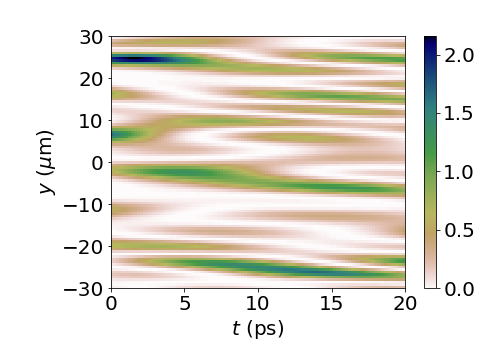
\includegraphics[width=0.4\textwidth]{ESSD_yt_m3.png}
         &  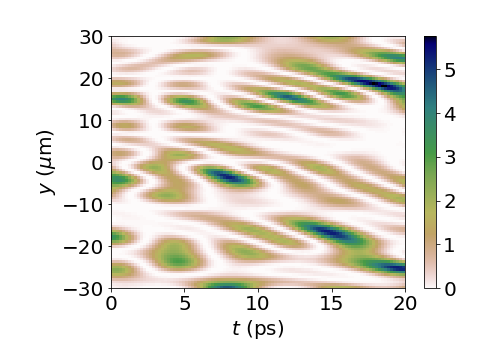
\includegraphics[width=0.4\textwidth]{ESSD_yt_m10.png} \\
         (c) $m=3$, $f_{T,z}$ &  (d) $m=10$, $f_{T,z}$   \\
            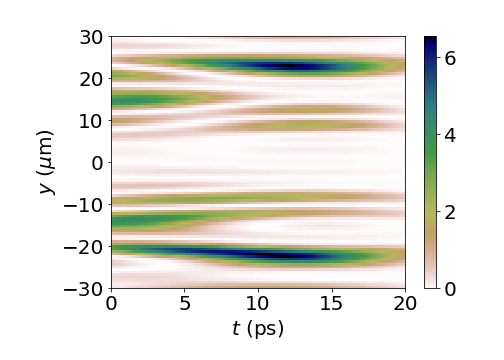
\includegraphics[width=0.4\textwidth]{ESSD_yt_m3_ft0.png}
         &  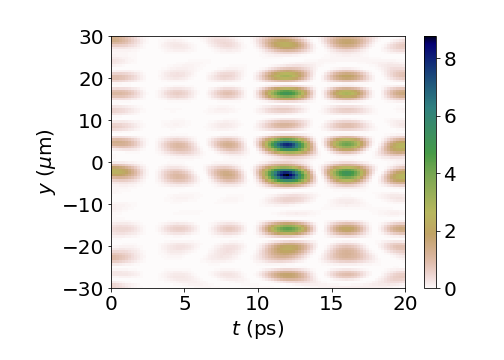
\includegraphics[width=0.4\textwidth]{ESSD_yt_m10_ft0.png}
    \end{tabular}
    \caption{Envelope field spatio-temporal evolution of RPP  laser with a $y$-aligned  [Eq. \eqref{eq:fty}] (a,b) and $z$-aligned  [Eq. \eqref{eq:ftz}] (c,d) transverse spectral  dispersion and of field given by  \eqref{eq:essd}, normalized to $E_0$ for $\lambda_0=0.35\, \mu m$, $f_\sharp = 8$, $N=100$, $\omega_m =2\pi\times  14.25\, \rm GHz$. }
    \label{fig:essd}
\end{figure*}

\subsection{General dispersion relation}
Hence, plugged into Eq. \eqref{eq:fd},  and in Maxwell equations linearized around the scattered field amplitude, $\delta E(\omega_d,\mathbf{k}_d) $, we obtain
\begin{align}
   \frac{\delta n_e }{n_{e0}}(\omega_s,\mathbf{k}_s) = -\alpha_{k/f}(v_\phi) \frac{A_k\epsilon_0 E_0}{N^{D-1} n_c T_e}   \sum_{l} \sum_{\mathbf{n}}  J_l(m) \left[  
     e^{i \Psi(\mathbf{n},l)} \delta E (\omega_s-\omega_l, \mathbf{k}_s-\mathbf{k}_{0,\mathbf{n},l})  
   +e^{-i \Psi(\mathbf{n},l)  } \delta E(\omega_s+\omega_l, \mathbf{k}_s+\mathbf{k}_{0,\mathbf{n},l})
   \right]
   \, ,\label{eq:fssd} 
\end{align}
and  
\begin{align}
    (\omega_d^2 - \omega_{pe}^2 -\mathbf{k}_d^2c^2)\delta E(\omega_d,\mathbf{k}_d) =& \frac{\omega_0^2}{2N^{D-1}} E_0 \sum_l\sum_{\mathbf{n}  }  J_l(m)  \times \nonumber \\ &\left[
    e^{i\Psi(\mathbf{n},l)}\frac{\delta n_e }{n_c}(\omega_d-\omega_l, \mathbf{k}_d-\mathbf{k}_{0,\mathbf{n},l})
    +e^{-i\Psi(\mathbf{n},l)}\frac{\delta n_e }{n_c}(\omega_d+\omega_l, \mathbf{k}_d+\mathbf{k}_{0,\mathbf{n},l}) \right] \, ,\label{eq:maxssd}
\end{align}
respectively.

Combining the two above equations and dropping the terms $\delta n_e(\omega_s \pm 2 \omega_l) $ arguing that  $\omega_l\sim \omega_0 \gg \omega _s$, four sums will appear, two running on the phase plate elements ($\mathbf{n}_1$, $\mathbf{n}_2$), and two on the SSD mode index, ($l_1$, $l_2$), thus giving
\begin{align}
   \frac{\delta n_e }{n_{e0}}(\omega_s,\mathbf{k}_s) &= -\alpha_{k/f}(v_\phi)\frac{n_{e0}}{n_c} \frac{A_k\epsilon_0 E_0}{N^{D-1} n_c T_e}\frac{\omega_0^2}{2N^{D-1}} E_0 \sum_{l_1} \sum_{l_2} \sum_{\mathbf{n}_1}    \sum_{\mathbf{n}_2}    J_{l_1}(m)J_{l_2}(m)\times  \nonumber \\
  & \Big[  
     \frac{e^{i \Psi(\mathbf{n}_1,l_1)-i \Psi(\mathbf{n}_2,l_2)}}{D_-}\frac{\delta n_e }{n_{e0}}  (\omega_s-\omega_{l_1}+\omega_{l_2},\mathbf{k}_s-\mathbf{k}_{0,\mathbf{n}_1,l_1}+\mathbf{k}_{0,\mathbf{n}_2,l_2})\nonumber\\
   & + \frac{e^{-i \Psi(\mathbf{n}_1,l_1)+i \Psi(\mathbf{n}_2,l_2)  }}{D_+} \frac{\delta n_e }{n_{e0}}(\omega_s+\omega_{l_1}-\omega_{l_2},\mathbf{k}_s+\mathbf{k}_{0,\mathbf{n}_1,l_1}-\mathbf{k}_{0,\mathbf{n}_2,l_2})
   \Big]
   \, ,\label{eq:fssd2} \\
   D_\pm &= (\omega_s\pm\omega_{l_1})^2 - \omega_{pe}^2 -(\mathbf{k}_s\pm\mathbf{k}_{0,\mathbf{n}_1,l_1})^2c^2 \, .
\end{align}
The simplification of this equation may be carried, by applying a statistical averaged and using Eq. \eqref{eq:d}, giving, 
 \begin{equation}\label{eq:d2}
 \langle e^{i \Psi(\mathbf{n}_1,l_1)-i \Psi(\mathbf{n}_2,l_2) }\rangle=
  e^{iT_{r} \omega_{l_1}f_{T/L}[\mathbf{k}_\perp(\mathbf{n}_1,l_1)]  }
  e^{-iT_{r}  \omega_{l_2}f_{T/L}[\mathbf{k}_\perp(\mathbf{n}_1,l_2)]  }
 \delta(\mathbf{n}_1-\mathbf{n}_2) \, ,
 \end{equation}
and thus,
\begin{align}
   \frac{\delta n_e }{n_{e0}}(\omega_s,\mathbf{k}_s) &= -\alpha_{k/f}(v_\phi) \frac{n_{e0}}{n_c} \frac{A_k\epsilon_0 E_0}{N^{D-1} n_c T_e}\frac{\omega_0^2}{2} E_0  \sum_{l_1}  \sum_{l_2} \sum_{\mathbf{n}}    J_{l_1}(m)J_{l_2}(m) \times \nonumber \\
  & \Big[  
     \frac{  e^{iT_{r} \omega_{l_1}f_{T/L}[\mathbf{k}_\perp(\mathbf{n},l_1)]  }
  e^{-iT_{r}  \omega_{l_2}f_{T/L}[\mathbf{k}_\perp(\mathbf{n},l_2)]  }
     }{(\omega_s-\omega_{l_1})^2 - \omega_{pe}^2 -(\mathbf{k}_s- \mathbf{k}_{0,\mathbf{n},l_1})^2c^2}
     \frac{\delta n_e }{n_{e0}}  (\omega_s-\omega_{l_1}+\omega_{l_2},\mathbf{k}_s-\mathbf{k}_{0,\mathbf{n},l_1}+\mathbf{k}_{0,\mathbf{n},l_2})\nonumber\\&
   + \frac{   e^{-iT_{r} \omega_{l_1}f_{T/L}[\mathbf{k}_\perp(\mathbf{n},l_1)]  }
  e^{iT_{r}  \omega_{l_2}f_{T/L}[\mathbf{k}_\perp(\mathbf{n},l_2)]  }
   }{(\omega_s+\omega_{l_1})^2 - \omega_{pe}^2 -(\mathbf{k}_s+ \mathbf{k}_{0,\mathbf{n},l_1})^2c^2} 
   \frac{\delta n_e }{n_{e0}}(\omega_s+\omega_{l_1}-\omega_{l_2},\mathbf{k}_s+\mathbf{k}_{0,\mathbf{n},l_1}-\mathbf{k}_{0,\mathbf{n},l_2}) 
   \Big]
   \, .\label{eq:fssd3}
\end{align}
In order to further simplify the dispersion relation, we will address the growth of a monochromatic acoustic wave  of frequency $\Bar{\omega_s}$ and wavevector $\Bar{\mathbf{k}_s}$ so that $\delta n_e/n_{e0}\propto \delta(\omega_s-\Bar{\omega_s}, {\mathbf{k}_s}-\Bar{\mathbf{k}_s})$. Hence    with $\delta n_0/n_{c} =(n_{e0}/n_c)\epsilon_0 E_0^2/ (2n_c T_e ) $
\begin{align}
   \delta(\omega_s-\Bar{\omega_s}, {\mathbf{k}_s}-\Bar{\mathbf{k}_s})
   &= -A_k \frac{\delta n_0}{n_c}\frac{\omega_0^2}{N^{D-1}}  \sum_{l_1}  \sum_{l_2} \sum_{\mathbf{n}}    J_{l_1}(m)J_{l_2}(m)\alpha_{k/f}\left(\frac{\omega_s}{\vert\mathbf{k}_s \vert} \right) \times \nonumber \\
  & \Big[  
     \frac{  e^{iT_{r} \omega_{l_1}f_{T/L}[\mathbf{k}_\perp(\mathbf{n},l_1)]  }
  e^{-iT_{r}  \omega_{l_2}f_{T/L}[\mathbf{k}_\perp(\mathbf{n},l_2)]  }
     }{(\omega_s-\omega_{l_1})^2 - \omega_{pe}^2 -(\mathbf{k}_s- \mathbf{k}_{0,\mathbf{n},l_1})^2c^2}
     \delta(\omega_s-\omega_{l_1}+\omega_{l_2}-\Bar{\omega_s}, \mathbf{k}_s-\mathbf{k}_{0,\mathbf{n},l_1}+\mathbf{k}_{0,\mathbf{n},l_2}-\Bar{\mathbf{k}_s}) \nonumber\\&
   + \frac{   e^{-iT_{r} \omega_{l_1}f_{T/L}[\mathbf{k}_\perp(\mathbf{n},l_1)]  }
  e^{iT_{r}  \omega_{l_2}f_{T/L}[\mathbf{k}_\perp(\mathbf{n},l_2)]  }
   }{(\omega_s+\omega_{l_1})^2 - \omega_{pe}^2 -(\mathbf{k}_s+ \mathbf{k}_{0,\mathbf{n},l_1})^2c^2} 
    \delta(\omega_s+\omega_{l_1}-\omega_{l_2}-\Bar{\omega_s}, \mathbf{k}_s+\mathbf{k}_{0,\mathbf{n},l_1}-\mathbf{k}_{0,\mathbf{n},l_2}-\Bar{\mathbf{k}_s}) 
   \Big]
   \, .\label{eq:fssd3}
\end{align}

After an integration over $\omega_s$ and $\mathbf{k}_s$, we obtain,
\begin{align}
   1& = -A_k \frac{\delta n_0}{n_c}\frac{\omega_0^2}{N^{D-1}
   } 
    \sum_{l_1}  \sum_{l_2} \sum_{\mathbf{n}}    J_{l_1}(m)J_{l_2}(m)\times \nonumber \\
  & \Big[  
  \alpha_{k/f}\left(\frac{\Bar{\omega_s}+\omega_{l_1}-\omega_{l_2}}
 %
  {\vert\Bar{\mathbf{k}_s}+\mathbf{k}_{0,\mathbf{n},l_1}-\mathbf{k}_{0,\mathbf{n},l_2} \vert}
  %
  %
  \right) 
     \frac{  e^{iT_{r} \omega_{l_1}f_{T/L}[\mathbf{k}_\perp(\mathbf{n},l_1)]  }
  e^{-iT_{r}  \omega_{l_2}f_{T/L}[\mathbf{k}_\perp(\mathbf{n},l_2)]  }
     }{(\Bar{\omega_s}-\omega_{l_2})^2 - \omega_{pe}^2 -(\Bar{\mathbf{k}_s}- \mathbf{k}_{0,\mathbf{n},l_2})^2c^2}
      \nonumber\\&
   +\alpha_{k/f}\left(\frac{\Bar{\omega_s}-\omega_{l_1}+\omega_{l_2}}
   %
   {\vert\Bar{\mathbf{k}_s}-\mathbf{k}_{0,\mathbf{n},l_1}+\mathbf{k}_{0,\mathbf{n},l_2}-\vert} 
   %
   %
   \right)  \frac{   e^{-iT_{r} \omega_{l_1}f_{T/L}[\mathbf{k}_\perp(\mathbf{n},l_1)]  }
  e^{iT_{r}  \omega_{l_2}f_{T/L}[\mathbf{k}_\perp(\mathbf{n},l_2)]  }
   }{(\Bar{\omega_s}+\omega_{l_2})^2 - \omega_{pe}^2 -(\Bar{\mathbf{k}_s}+ \mathbf{k}_{0,\mathbf{n},l_2})^2c^2} 
   \Big]
   \, .\label{eq:fssd4}
\end{align}

In order to reach analytical progress, we may now simplify the denominators in the square bracket,   using $\omega_l^2 = \omega_{pe}^2 +\mathbf{k}_{0,\mathbf{n},l}^2c^2$  and $\omega_s^2\ll \mathbf{k}_s^2c^2$ while replacing  $\Bar{\omega_s},\Bar{\mathbf{k}_s}$   by ${\omega_s},\mathbf{k}_s$,
\begin{equation}
    (\omega_s\pm\omega_{l_2})^2 - \omega_{pe}^2 -(\mathbf{k}_s\pm \mathbf{k}_{0,\mathbf{n},l_2})^2c^2 \simeq  - \mathbf{k}_s^2c^2 \pm2(\omega_s\omega_{l_2} - \mathbf{k}_s \cdot \mathbf{k}_{0,n,l_2}) \, .
\end{equation}
We will also use,
\begin{align}
    \mathbf{k}_{0,\mathbf{n},l_1}-\mathbf{k}_{0,\mathbf{n},l_2}&=
    %k_{l_1}\Hat{\mathbf{x}}-k_{l_2}\Hat{\mathbf{x}} + \mathbf{k}_\perp(\mathbf{n}_1,l_1)-\mathbf{k}_\perp(\mathbf{n}_1,l_2) = 
    k_0\frac{\omega_m}{\omega_0}(l_1-l_2)\Hat{\mathbf{x}} +\frac{2k_m}{N} \frac{\omega_m}{\omega_0}(l_1-l_2)\mathbf{n}%\equiv(l_1-l_2) \Delta\mathbf{k}\,,
    \nonumber\\&
    \simeq  k_0\frac{\omega_m}{\omega_0}(l_1-l_2)\Hat{\mathbf{x}} \, ,
\end{align}
thus giving,
\begin{align}
   1& = -A_k \frac{\delta n_0}{n_c}\frac{\omega_0^2}{N^{D-1}} 
    \sum_{l_1, l_2} 
     J_{l_1}(m)J_{l_2}(m) %\nonumber \\&
    \Big[  
  \alpha_{k/f}\left(\frac{\omega_s+(l_1-l_2)\omega_m}
 %
  {\vert\mathbf{k}_s+(l_1-l_2)k_0\omega_m/\omega_0\Hat{\mathbf{x}} \vert}
  %
  %
  \right)  \sum_{\mathbf{n}}  
     \frac{  e^{iT_{r} \omega_{l_1}f_{T/L}[\mathbf{k}_\perp(\mathbf{n},l_1)]  }
  e^{-iT_{r}  \omega_{l_2}f_{T/L}[\mathbf{k}_\perp(\mathbf{n},l_2)]  }
     }{ - \mathbf{k}_s^2c^2 -2(\omega_s\omega_{l_2} - \mathbf{k}_s \cdot \mathbf{k}_{0,n,l_2}c^2)}
      \nonumber\\&
   +\alpha_{k/f}\left(\frac{\omega_s-(l_1-l_2)\omega_m}
   %
   {\vert\mathbf{k}_s-(l_1-l_2)k_0\omega_m/\omega_0\Hat{\mathbf{x}} \vert} 
   %
   %
   \right)  \sum_{\mathbf{n}}   \frac{   e^{-iT_{r} \omega_{l_1}f_{T/L}[\mathbf{k}_\perp(\mathbf{n},l_1)]  }
  e^{iT_{r}  \omega_{l_2}f_{T/L}[\mathbf{k}_\perp(\mathbf{n},l_2)]  }
   }{ - \mathbf{k}_s^2c^2 +2(\omega_s\omega_{l_2} - \mathbf{k}_s \cdot \mathbf{k}_{0,n,l_2}c^2)} 
   \Big] 
   \, .\label{eq:fssd5}
\end{align}
In order to facilitate the resolution, we will only account for the leading terms in $\omega_m/\omega_0$, which for most laser facilities verifies $\omega_m/\omega_0\lesssim 10^{-4}$. We will therefore derive the following to leading order in $\omega_m/\omega_0$, giving $\omega_l \simeq \omega_0$ and $\mathbf{k}_{0,n,l} \simeq \mathbf{k}_{0,n,0}\equiv \mathbf{k}_{0,n}$. Likewise,  $iT_{r} \omega_{l_1}f_{T/L}[\mathbf{k}_\perp(\mathbf{n},l_1)]  
  -iT_{r}  \omega_{l_2}f_{T/L}[\mathbf{k}_\perp(\mathbf{n},0)] 
  \simeq iT_{r}f_{T/L}[\mathbf{k}_\perp(\mathbf{n},l_2)]  (l_1-l_2) \omega_m/\omega_0 $.
  We thus obtain, 
  \begin{align}
   1& = -A_k \frac{\delta n_0}{n_c}\frac{\omega_0^2}{N^{D-1}} 
    \sum_{l_1,l_2} 
     J_{l_1}(m)J_{l_2}(m) %\nonumber \\&
    \Big[  
  \alpha_{k/f}\left(\frac{\omega_s+(l_1-l_2)\omega_m}
 %
  {\vert\mathbf{k}_s+(l_1-l_2)k_0\omega_m/\omega_0\Hat{\mathbf{x}} \vert}
  %
  %
  \right)  \sum_{\mathbf{n}}  
     \frac{  e^{ iT_{r}f_{T/L}[\mathbf{k}_\perp(\mathbf{n},0)]  (l_1-l_2) \omega_m/\omega_0  }
     }{ - \mathbf{k}_s^2c^2 -2(\omega_s\omega_{0} - \mathbf{k}_s \cdot \mathbf{k}_{0,n}c^2)}
      \nonumber\\&
   +\alpha_{k/f}\left(\frac{\omega_s-(l_1-l_2)\omega_m}
   %
   {\vert\mathbf{k}_s-(l_1-l_2)k_0\omega_m/\omega_0\Hat{\mathbf{x}} \vert} 
   %
   %
   \right)  \sum_{\mathbf{n}}   \frac{   e^{- iT_{r}f_{T/L}[\mathbf{k}_\perp(\mathbf{n},0)]  (l_1-l_2) \omega_m/\omega_0  }
   }{ - \mathbf{k}_s^2c^2 +2(\omega_s\omega_{0} - \mathbf{k}_s \cdot \mathbf{k}_{0,n}c^2)} 
   \Big] 
   \, .\label{eq:fssd6}
\end{align}

For a large enough number of diffracting elements, we shall use $N^{1-D}\sum_\mathbf{n} \equiv (2k_m)^{-2} \mathrm{PV} \int d\mathbf{k}_\perp  \times  $ where the integration runs over the domain $[-k_m,k_m]^{D-1}$ and $ \mathrm{PV}$ designates the principal value.
This results in,
  \begin{align}
   1& = -\frac{A_k}{4k_m^2} \frac{\delta n_0}{n_c}\omega_0^2
    \sum_{l_1,l_2} 
     J_{l_1}(m)J_{l_2}(m) %\nonumber \\&
    \Big[  
  \alpha_{k/f}\left(\frac{\omega_s+(l_1-l_2)\omega_m}
 %
  {\vert\mathbf{k}_s+(l_1-l_2)k_0\omega_m/\omega_0\Hat{\mathbf{x}} \vert}
  %
  %
  \right)  \mathrm{PV} \int d\mathbf{k}_\perp 
     \frac{  e^{ iT_{r}f_{T/L}[\mathbf{k}_\perp]  (l_1-l_2) \omega_m }
     }{D_-}
      \nonumber\\&
   +\alpha_{k/f}\left(\frac{\omega_s-(l_1-l_2)\omega_m}
   %
   {\vert\mathbf{k}_s-(l_1-l_2)k_0\omega_m/\omega_0\Hat{\mathbf{x}} \vert} 
   %
   %
   \right) \mathrm{PV} \int d\mathbf{k}_\perp  \frac{   e^{- iT_{r}f_{T/L}[\mathbf{k}_\perp ]  (l_1-l_2) \omega_m  }
   }{D_+} 
   \Big] 
   %%%%%%%%%%%%%%%%%%%%%%%%%%%%%%%%%%%%
   \, ,\label{eq:fssd6} \\
   D_\pm &= - \mathbf{k}_s^2c^2 \pm2[\omega_s\omega_{0} - \mathbf{k}_s \cdot( k_0\Hat{\mathbf{x}} +\mathbf{k}_\perp)c^2] 
\end{align}

Note that when removing the $\sum_{l_1\neq l_2}$-terms from the above equation (keeping only $l_1=l_2$), and for $m$ larger than a few unity so that $\sum_{l=-m}^{l=m}J_l^2(m) \simeq 1$, the resulting dispersion relation coincides with the purely RPP case of Ref. \cite[]{Ruyer_FSBS}. Hence, the $l_1\neq l_2$-terms of the right-hand side of Eq. \eqref{eq:fssd6} enclose the influence of the spectral dispersion on the growth of the forward scatter. 

We will now assume the acoustic wavevector to lie in the $(x,y)$-plane, $\mathbf{k}_s = k_{s,x}\Hat{\mathbf{x}} +k_{s,y}\Hat{\mathbf{y}}$.
The outcome of the  terms $l_1\neq l_2$ depend on the nature of the spectral dispersion that is used (either longitudinal or transverse in the study). The longitudinal spectral dispersion has  an isotropic  delay function [see Eq. \eqref{eq:fl}] which implies that the growth of the forward scatter does not depend on the orientation of the acoustic wavevector in the transverse plane, \emph{i.e.} the growth of the scattered wave should be symmetric around the $x$-axis.  
Regarding the transverse SSD however, the dispersion relation varies whether we assume the  delay function axis [$y$-axis for  Eq. \eqref{eq:fty} and $z$-axis for  Eq. \eqref{eq:ftz}] to be normal to, or to lie into the $(\mathbf{k}_s,\mathbf{k}_0)$-plane [\emph{i.e.} $(x,y)$-plane].  

\section{Growth of a forward Brillouin scatter with a transverse spectral dispersion}
\subsection{Acoustic wavevector normal to the transverse SSD axis}\label{sec:ssdtz}
In this section we will analyse the simplest analytical case of a transverse SSD of axis normal to the acoustic wavevector [\emph{i.e.} using Eq. \eqref{eq:ftz}]. 
Hence, the  quadratures of Eq. \eqref{eq:fssd6} reads, 
\begin{align}
 \int d\mathbf{k}_\perp 
     \frac{  e^{ \pm  iT_{r}f_{T/L}[\mathbf{k}_\perp]  (l_1-l_2) \omega_m }
     }{D_\mp}=  e^{\pm iT_{r} (l_1-l_2)\frac{ \omega_m}{2} }
      \int_{-k_m}^{k_m} dk_{\perp,y} \int_{-k_m}^{k_m} dk_{\perp,z}\frac{  \exp\left( \pm  iT_{r}  (l_1-l_2)\omega_m \frac{k_{\perp,z}}{2k_m}  \right)
     }{- \mathbf{k}_s^2c^2 \mp 2(\omega_s\omega_{0} - k_{s,x}   k_0 c^2 - k_{s,y} k_{\perp,y} c^2) }
   \, ,\label{eq:int1}  \nonumber \\
   =  \pm \frac{ k_m}{k_{s,y} c^2} e^{ \pm iT_{r} (l_1-l_2)\frac{ \omega_m}{2} }
      \mathrm{sinc}\left(  T_{r}  (l_1-l_2) \omega_m/2  \right)
    \ln\left[\frac{- \mathbf{k}_s^2c^2\mp 2(\omega_s\omega_{0} - k_{s,x}   k_0 c^2  - k_{s,y} k_m c^2)}
    {- \mathbf{k}_s^2c^2\mp 2(\omega_s\omega_{0} - k_{s,x}   k_0  c^2 + k_{s,y} k_m c^2)}\right]\, ,
\end{align}
where we introduced the sinus cardinal function, $ \mathrm{sinc}(x)=\sin(x)/x$.
Equation \eqref{eq:fssd6} thus becomes
 \begin{align}
   1 =& -\frac{A_k}{4k_mk_{s,y} c^2} \frac{\delta n_0}{n_c}\omega_0^2
    \sum_{l_1, l_2} 
     J_{l_1}(m)J_{l_2}(m)
      \mathrm{sinc}\left(  T_{r}  (l_1-l_2) \omega_m/2  \right)\times \Big\{
      \nonumber \\&
      e^{ + iT_{r} (l_1-l_2)\frac{ \omega_m}{2} }
  \alpha_{k/f}\left(\frac{\omega_s+(l_1-l_2)\omega_m}
  {\vert\mathbf{k}_s+(l_1-l_2)k_0\omega_m/\omega_0\Hat{\mathbf{x}} \vert}
  \right)   
  \ln\left[\frac{- \mathbf{k}_s^2c^2-2(\omega_s\omega_{0} - k_{s,x}   k_0 c^2  - k_{s,y} k_m c^2)}
    {- \mathbf{k}_s^2c^2 -2(\omega_s\omega_{0} - k_{s,x}   k_0 c^2  + k_{s,y} k_m c^2)}\right]
%%
     \nonumber \\&
      -e^{ - iT_{r} (l_1-l_2)\frac{ \omega_m}{2} }
  \alpha_{k/f}\left(\frac{\omega_s-(l_1-l_2)\omega_m}
  {\vert\mathbf{k}_s-(l_1-l_2)k_0\omega_m/\omega_0\Hat{\mathbf{x}} \vert}
  \right)   
  \ln\left[\frac{- \mathbf{k}_s^2c^2+2(\omega_s\omega_{0} - k_{s,x}   k_0 c^2  - k_{s,y} k_m c^2)}
    {- \mathbf{k}_s^2c^2 +2(\omega_s\omega_{0} - k_{s,x}   k_0 c^2  + k_{s,y} k_m c^2)}\right]
    \Big\}
   \, .\label{eq:fssd7}
   \end{align}

As in most spectral dispersion used, $\omega_mT_r = 2\pi $, the $\mathrm{sinc}$ of the above equation is vanishing for  $l_1\neq l_2$. When retaining $l_1=l_2$ in the sum, the above dispersion relation recovers the pure RPP limit. This demonstrates that the transverse SSD does not affect the growth of the  scatter  transversely to the phase shift direction. This not only concerns the growth the FSBS as mainly  addressed in this work, but also of the filamentation instability (when setting $\omega_s=0$). Hence, when the filamentation survives the use of RPP, as in a cold enough   or a multi-ion species plasma \cite[]{Ruyer_FSBS}, this instability should remain unaffected for wavevectors transverse to the SSDT direction.

\subsection{Acoustic wavevector parallel to the transverse SSD axis}\label{sec:ssdty}
When transverse SSD phase shift direction lies in the $(\mathbf{k}_s,\mathbf{k}_0)$-plane [\emph{i.e.} using Eq. \eqref{eq:fty}], the quadratures of Eq. \eqref{eq:fssd6} are still tractable. They give
\begin{align}
 \int d\mathbf{k}_\perp 
     \frac{  e^{ \pm  iT_{r}f_{T/L}[\mathbf{k}_\perp]  (l_1-l_2) \omega_m }
     }{D_\mp}&=  e^{\pm iT_{r} (l_1-l_2)\frac{ \omega_m}{2} }
      \int_{-k_m}^{k_m} dk_{\perp,z} \int_{-k_m}^{k_m} dk_{\perp,y}\frac{  \exp\left( \pm  iT_{r}  (l_1-l_2)\omega_m \frac{k_{\perp,y}}{2k_m}  \right)
     }{- \mathbf{k}_s^2c^2 \mp 2(\omega_s\omega_{0} - k_{s,x}   k_0 c^2 - k_{s,y} k_{\perp,y} c^2) }
   \, ,\label{eq:int1}  \nonumber \\
   &=2k_m e^{\pm iT_{r} (l_1-l_2)\frac{ \omega_m}{2} } F_T(a_\pm,b_\pm,c_\pm) \, .
\end{align}

Defining,
\begin{align}
    F_T(a,b,c)&= \int_{-k_m}^{k_m} \frac{e^{iax}}{b+cx}dx\, ,\\
\end{align}
we obtain,
\begin{align}
     F_T(a,b,c) &  = \frac{1}{c}\left[
    e^{-iab/c}\mathrm{Ei}\left(ia\frac{b+cx}{c}\right)
    \right]_{x=-k_m}^{x=+k_m}\, ,\label{eq:fabc}\\
    a_\pm&=\pm\frac{T_r\omega_m}{2k_m}(l_1-l_2)\, ,\label{eq:fa}\\
    b_\pm&=- \mathbf{k}_s^2c^2 \mp 2( \omega_s\omega_{0}-k_{sx}k_0c^2 )\, ,\label{eq:fb} \\
    c_\pm&=\pm 2 k_{s,y}c^2\, .\label{eq:fc}
\end{align}
We introduced $\mathrm{Ei}(x)$ the one-argument exponential integral function defined as the principle value of $\int_{-\infty}^x dt e^{t}/t$ \cite[]{Abramowitz}. 

In this case, the dispersion relation reads,
\begin{align}
   1 =& - \frac{A_k}{2k_m}  \frac{\delta n_0}{n_c}\omega_0^2
    \sum_{l_1, l_2} 
     J_{l_1}(m)J_{l_2}(m) 
      \Big[&
      %\nonumber \\&
       \alpha_{k/f}\left(\frac{\omega_s+(l_1-l_2)\omega_m}
  {\vert\mathbf{k}_s+(l_1-l_2)k_0\omega_m/\omega_0\Hat{\mathbf{x}} \vert}
  \right) 
      e^{ + iT_{r} (l_1-l_2)\frac{ \omega_m}{2} }  F_T(a_+,b_+,c_+)
%%
     \nonumber \\&
      + &\alpha_{k/f}\left(\frac{\omega_s-(l_1-l_2)\omega_m}
 %
  {\vert\mathbf{k}_s-(l_1-l_2)k_0\omega_m/\omega_0\Hat{\mathbf{x}} \vert}
  %
  %
  \right) 
      e^{ - iT_{r} (l_1-l_2)\frac{ \omega_m}{2} }   F_T(a_-,b_-,c_-)
    \Big]
   \, .\label{eq:fssdty}
\end{align}
   
For the laser and plasma parameters relevant for high energy laser facilities, no appropriate  approximations could be found to reach analytical resolution of the above dispersion relation. However, for vanishing value of $\vert \mathbf{k}_s \vert $, the influence of spectral dispersion is negligible  and the solution of Eq. \eqref{eq:fssdty} coincide with the pure RPP case [Eq. (27) of Ref. \cite[]{Ruyer_FSBS} or assuming $m=0$ in \eqref{eq:fssdty}]. Hence starting by   the pure RPP solution with vanishing ${k}_{s,y}$, the value $k_{s,x}({k}_{s,y}, \omega_s) $ that fulfills Eq. \eqref{eq:fssdty}  may be obtained for a given $\omega_s$ by using a non-linear algebraic numerical solver  with slowly increasing values of $k_{s,y}$.

\subsection{Longitudinal  spectral dispersion}\label{sec:ssdl}
The longitudinal spectral dispersion relation as used on LMJ, is characterized by a radial phase shift of the different frequency modes \cite[]{POP_Duluc_2019}. Combining the longitudinal phase shift function,  Eq. \eqref{eq:fl}, with the dispersion relation of Eq. \eqref{eq:fssd6}, gives \begin{align}
   1 =& - \frac{A_k}{4k_m^2}  \frac{\delta n_0}{n_c}\omega_0^2
    \sum_{l_1, l_2} 
     J_{l_1}(m)J_{l_2}(m) 
      \Big[&
      %\nonumber \\&
       \alpha_{k/f}\left(\frac{\omega_s+(l_1-l_2)\omega_m}
  {\vert\mathbf{k}_s+(l_1-l_2)k_0\omega_m/\omega_0\Hat{\mathbf{x}} \vert}
  \right) 
       F_L(a_+,b_+,c_+)
%%
     \nonumber \\&
      + &\alpha_{k/f}\left(\frac{\omega_s-(l_1-l_2)\omega_m}
  {\vert\mathbf{k}_s-(l_1-l_2)k_0\omega_m/\omega_0\Hat{\mathbf{x}} \vert}
  \right) 
     F_L(a_-,b_-,c_-)
    \Big]
   \, ,\label{eq:fssdl}
   \end{align}
with 
\begin{align}
    F_L(a_\pm,b_\pm,c_\pm)&= \int_{-k_m}^{k_m}dk_z\int_{-k_m}^{k_m} dk_y \frac{e^{ia_\pm(k_y^2 + k_z^2)}}{b_\pm+c_\pm k_y }\, ,
   % = -(-1)^{1/4}\sqrt{\frac{\pi}{a}} \mathrm{erf} \left( (-1)^{3/4}k_m\sqrt{a} \right)   \int_{-k_m}^{k_m} dk_y \frac{e^{iak_y^2}}{b+ck_y } \, . 
   %F_L(a,b,c)&= \int_{0}^{k_m}dx\int_{-\pi}^{\pi} d\theta \frac{xe^{iax}}{b+cx\cos(\theta) }\, ,
\end{align}
and
\begin{align}
    a_\pm&=\pm\frac{T_r\omega_m}{k_m}(l_1-l_2)\, ,\label{eq:fla}\\
    b_\pm&=- \mathbf{k}_s^2c^2 \mp 2(\omega_s\omega_{0}-k_{sx}k_0c^2) \, ,\label{eq:flb} \\
    c_\pm&=\pm 2 k_{s,y}c^2\, .\label{eq:flc}
\end{align}
A fairly compact formula may be obtained for $F_L$ provided one approximates $\exp[ia(k_z^2+k_y^2)]\simeq 1+ia(k_z^2+k_y^2)$. This also corresponds to replacing the longitudinal quadratic delay function, [Eq. \eqref{eq:fl}] by 
\begin{equation}\label{eq:fl_ap}
f_L(\mathbf{k}/k_m) = \log(1+\xi \mathbf{k}^2/k_m^2)\, ,
\end{equation}
with $\xi=1$. As detailed subsequently [in Sec. \ref{sec:sol}, Fig. \ref{fig:ssdl}], identical spatial growth rates are obtained when setting $\xi=1.6$ or using   $f_L(\mathbf{k}/k_m) = \vert \mathbf{k}\vert /k_m$.  Hence the modified longitudinal delay function   seems therefore to be a good approximate, leading to 
\begin{align}
    F_L(a_\pm,b_\pm,c_\pm)&=-4k_m^2 \frac{ia_\pm b_\pm}{2c_\pm^2} +\frac{2k_m}{c}\left(1+\frac{ia_\pm k_m^2}{3}+\frac{ia_\pm b_\pm^2}{c_\pm^2}\right) \log\left( \frac{b_\pm+c_\pm k_m}{b_\pm-c_\pm k_m}   \right) \, .
\end{align}
\end{widetext}
The resolution of the above equations is identical to the the case of Sec. \ref{sec:ssdty}.

\section{Comparison with hydrodynamic paraxial Hera simulations}
\subsection{Simulation setup}
In order to validate our developments, we performed hydrodynamic  paraxial Hera simulations \cite[]{Loiseau_2006}.

We used a 2D domain of size $L_x \times L_y = 2000 \times 1000\, \rm \mu$m$^2$. 
The beam propagates in the $x$-direction and is injected at the left boundary, $x_\mathrm{BC}=0$, with a  $\lambda_0=0.35\, \rm\mu m$-wavelength and an averaged intensity of $I_0=6\times 10^{14}\, \rm W/cm^2$.
The beam is focused at the center of the domain, at 
$x_\mathrm{foc}=1000\, \rm \mu m$ and $y_\mathrm{foc}=0$ with  $f_\sharp = 8$, and
a spatial and temporal envelope following
\begin{align}
    \hat{g}(y) &= \exp(-\vert y\vert ^o/2\sigma_g^o)  \, ,  \label{eq:g}\\
    h(t) &= \mathrm{min}(t/\tau_h,1) \, ,\label{eq:h}
\end{align}
respectively with $\tau_h=1\, \rm ps$,  $o=5$ and $\sigma_g = 200\,\rm \mu m$.  
Moreover, the bremsstrahlung energy deposition is neglected and we account for the non-local thermal correction of Eq. \eqref{eq:nl}.  
Moreover a barotropic gas is assumed  with $T_e=1\,\rm keV$ and $T_i=300\,\rm eV$, an electron density of $n_e =0.1n_c $ and outflow boundary for the fluid.
The mesh size is $dx =0.325\,\rm \mu m$, $dy = 0.0625\, \rm \mu m$
%and a timestep of $dt=10^{-13}$ s 
with a normalized Landau acoustic damping rate of \tc{$\gamma_0=0.16$} that corresponds to the collisional fit of Ref. \cite[]{casanova_1989}. 
The acoustic Landau damping operator is computed transversely to the laser direction in the Fourier space, as introduced in Ref. \cite[]{POP_Rose_96}, described in \cite[]{Berger_98} and used in   \cite{phd-PEML,Masson_2006,Huller_2008}.
Finally, for simplicity, we do no account for any back-scattering in our  simulations. 

\subsection{Solution of the dispersion relations and discussion }\label{sec:sol}
\begin{figure}
\begin{tabular}{c}
(a) Theory, SSDT \\
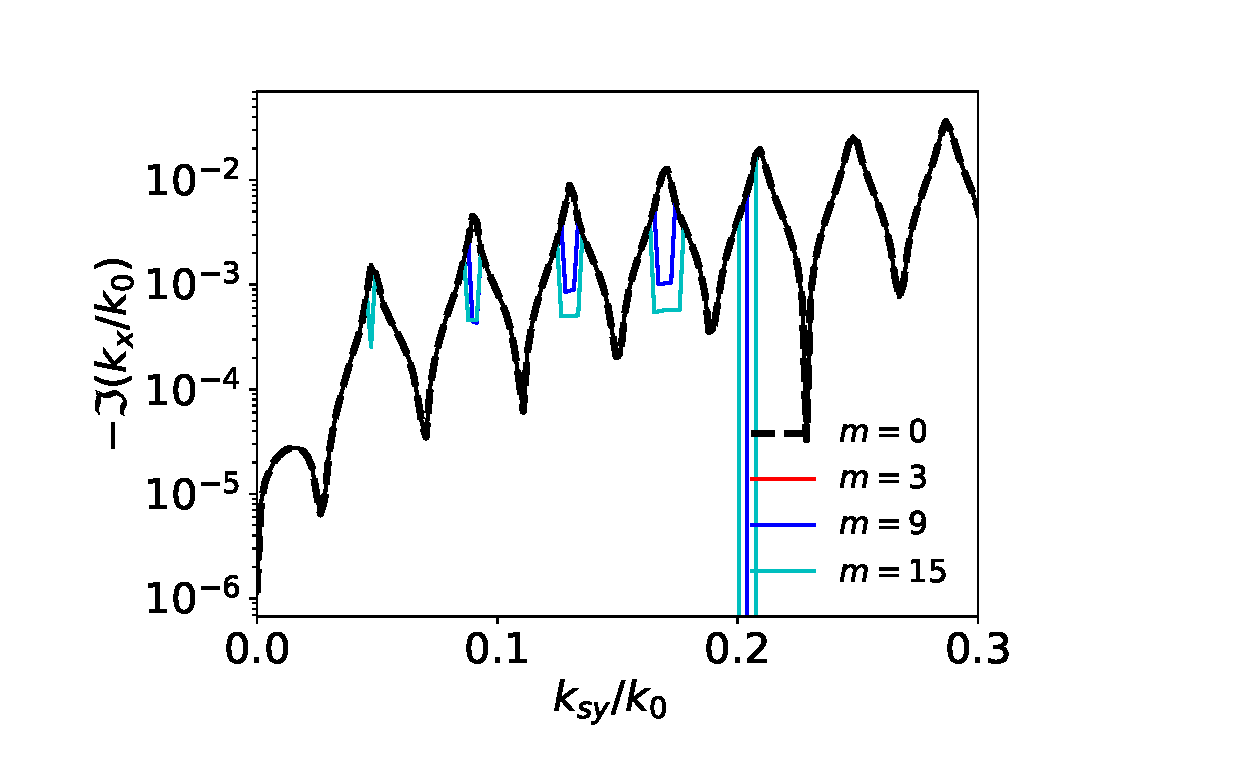
\includegraphics[width=0.45\textwidth,trim={-2cm 0 0 0},clip]{SSD_H+1keV300eV.eps}\\
(b) HERA, SSDT \\
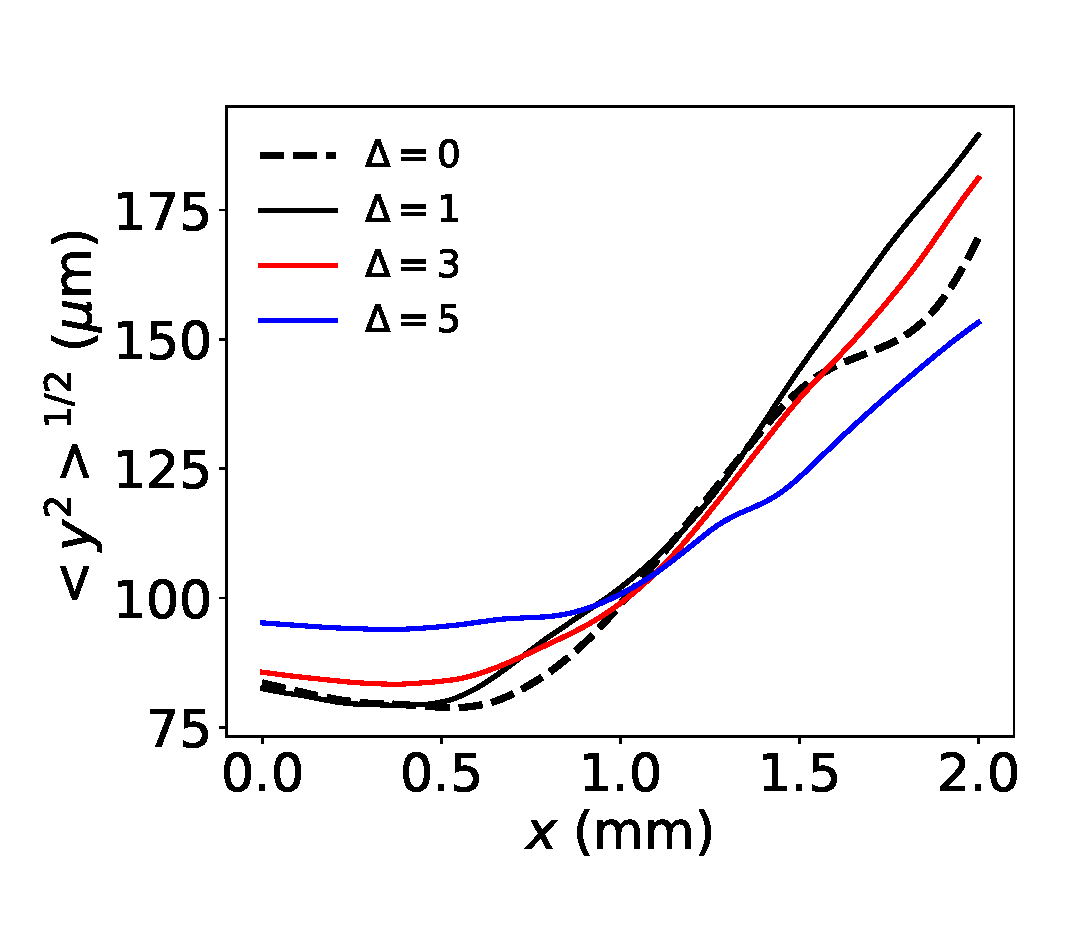
\includegraphics[width=0.35\textwidth]{FSBS_SSD_waist_100ps.eps}
\end{tabular}
\caption{ \label{fig:ssdt} 
Spatial growth rate in the $y$ direction of the forward Brillouin instability for an averaged laser intensity and wavelength $I_0=6\times 10^{14}\,\rm W/cm^2$ and  $\lambda_0=0.35\,\mu m$ and a  H$^+$  plasma with $T_e =1\,\rm  keV$, $ T_i=300\,  \rm eV$  and $n_{e}=0.1n_c$.
The RPP uses $f_\sharp = 8$ and a $y$-aligned transverse SSD [Eq. \eqref{eq:fssdty}] with $\omega_m=2\pi \times14.25\,\rm GHz$ and a $m$-number ranging from $0$ (no temporal smoothing) to $15$.
The black plain line corresponds to 
A  $z$-aligned transverse SSD [thus transverse to the spatial growth direction, Eq. \eqref{eq:fssd7}] with $m=33$ is superimposed as a black thin plain line. 
(b) Transverse waist defined as $\langle y^2\rangle=\int dyI(y)y^2 /\int dyI(y)$ as a function of $x$  from the SSDT HERA   simulations at $t=100\,\rm ps$.
}
\end{figure}

\begin{figure}
\begin{tabular}{c}
(a) $m=0$\\
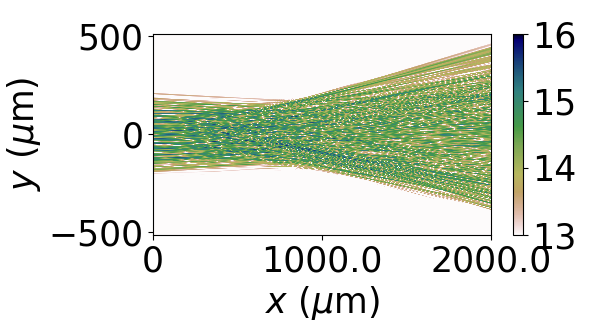
\includegraphics[width=0.4\textwidth,trim={2cm 0 0 0},clip]{ISSD0.png}\\
(b)  $m=3$\\
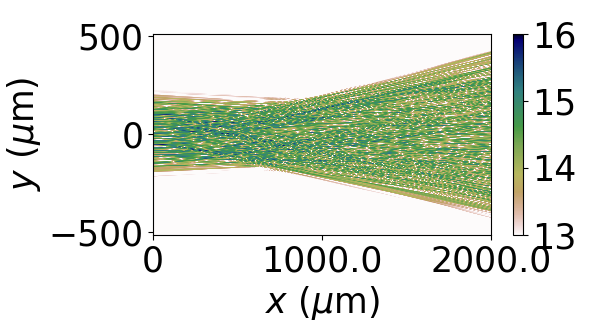
\includegraphics[width=0.4\textwidth,trim={2cm 0 0 0},clip]{ISSD1.png}\\
%(b) HERA, $m=9$\\
%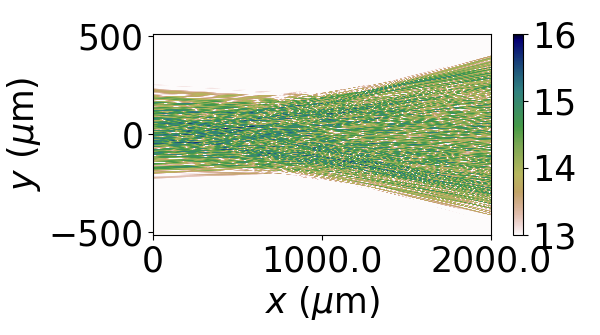
\includegraphics[width=0.45\textwidth,trim={2cm 0 0 0},clip]{ISSD3.png}\\
(c) $m=15$\\
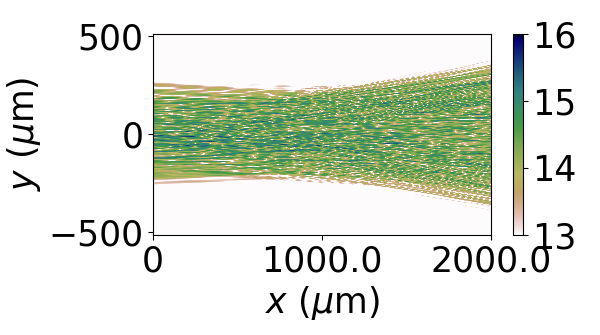
\includegraphics[width=0.4\textwidth,trim={2cm 0 0 0},clip]{ISSD5.png}
\end{tabular}
\caption{ \label{fig:ssdt_I} 
  Intensity profile resulting from HERA paraxial simulations with transverse SSD at $t=100\,\rm ps$. The plasma and laser parameters are detailed in Fig. \ref{fig:ssdt}.
}
\end{figure}
Figure \ref{fig:ssdt}(a) illustrates the density fluctuations spatial growth rate of the forward Brillouin instability in the $y$ direction  for a $y$-transversely smoothed laser beam. As shown in Ref. \cite[]{Ruyer_FSBS}, the FSBS growth lies on the acoustic trace so that Fig.  \ref{fig:ssdt}(a) corresponds to acoustic frequencies $\omega_s=k_yc_s$.   First of all, we assess that using $z$-aligned transverse smoothing (solving Eq. \eqref{eq:fssd7}, as a thin black plain line) gives the same results that without SSD (black dashed line), thus confirming the conclusions of Sec. \ref{sec:ssdtz}: the transverse $z$-aligned temporal smoothing has no effect on the  FSBS spatial growth of acoustic fluctuations propagating in the $y$ direction. 
However, the solutions of Eq. \eqref{eq:fssdty}, as colored plain lines, evidence a decrease of the first peaks of the  spatial FSBS growth rate. Figure \ref{fig:ssdt}(a) shows that the increase of the mode number tends to decrease the first maximums, reducing by more than a factor two the growth rate  for $m= 15$.
However, the peak number six and seven (at $k_s\gtrsim0.2k_0$) are   weakly or not affected by the temporal smoothing. 
The propagation of the corresponding laser pulse in a paraxial hydrodynamic simulation code such as HERA \cite[]{Loiseau_2006},
results in a significant increase of the beam aperture, and  nearly independent of the spectral dispersion strength, as illustrated in Figs. \ref{fig:ssdt_I}(a,b,c).
As shown in Ref. \cite[]{Ruyer_FSBS}, the first acoustic wave to reach saturation for $m=0$ in  Fig. \ref{fig:ssdt} (\emph{i.e.} without SSD, black dashed line), may be related to the maximum of the scattered intensity and reads $k_s\simeq 0.27 k_0$. As the corresponding growth peak is unaffected by the spectral dispersion, one does not expect a significant effect of SSD on the propagation of the beam, which is  confirmed by Figs. \ref{fig:ssdt_I}(a,b,c). 

The transverse waist of the beam, illustrated in Fig. \ref{fig:ssdt}(b) for $t=100\, \rm ps$ for different mode numbers, demonstrates that $m=0$, $3$ and $9$ leads to similar results, with a waist of $\sim 175\,\rm\mu m$ after $2\,\rm mm$ of propagation. For $m=15$ however, a somewhat smaller waist of $\sim 150\,\rm\mu m$ is obtained and can be ascribed to the larger waist characterized at $x=0$ by our simulation results. 
Indeed, for large values of  $m$, the off-focus waist is found to slightly increase (here by about 10\%) leading to a smaller average intensity and therefore, smaller FSBS growth rate and aperture increase. 
\tc{
Such dependence  of the off-focus waist on $m$ is not accounted  for in our analysis as we reduced the phase plate elements to monochromatic contributions in Eq. \eqref{eq:essd} [or Dirac functions in Eq. \eqref{eq:essdwk}]. Hence, in our case, the spatial growth rate and the laser waist both remain independent of $m$. 
Interestingly, we may counterbalance the decrease of $I_0$ (and the increase of the waist) by    decreasing the  laser waist by 10\% while  increasing the averaged intensity  by the same amount in our $m=15$-simulation. The resulting waist profile,  illustrated by the dashed blue line in Fig. \ref{fig:ssdt}(b), matches the $m=0$, $3$, $9$ cases thus confirming the predictability of our dispersion relations, even at large SSDT-strength, provided the effective averaged intensity is known.
}

\begin{figure}
\begin{tabular}{c}
(a) Theory\\
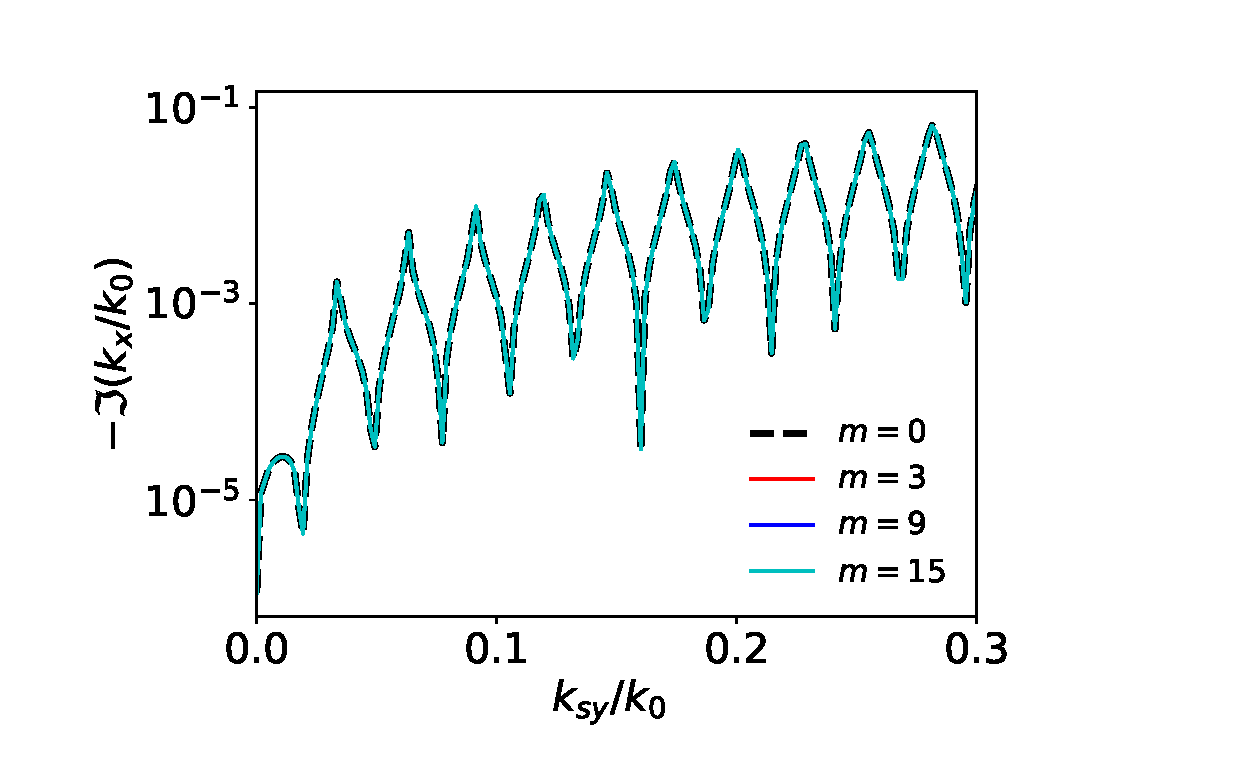
\includegraphics[width=0.45\textwidth,trim={-2cm 0 0 0},clip]{SSDL_H+1keV300eV.eps}\\
(b) HERA \\
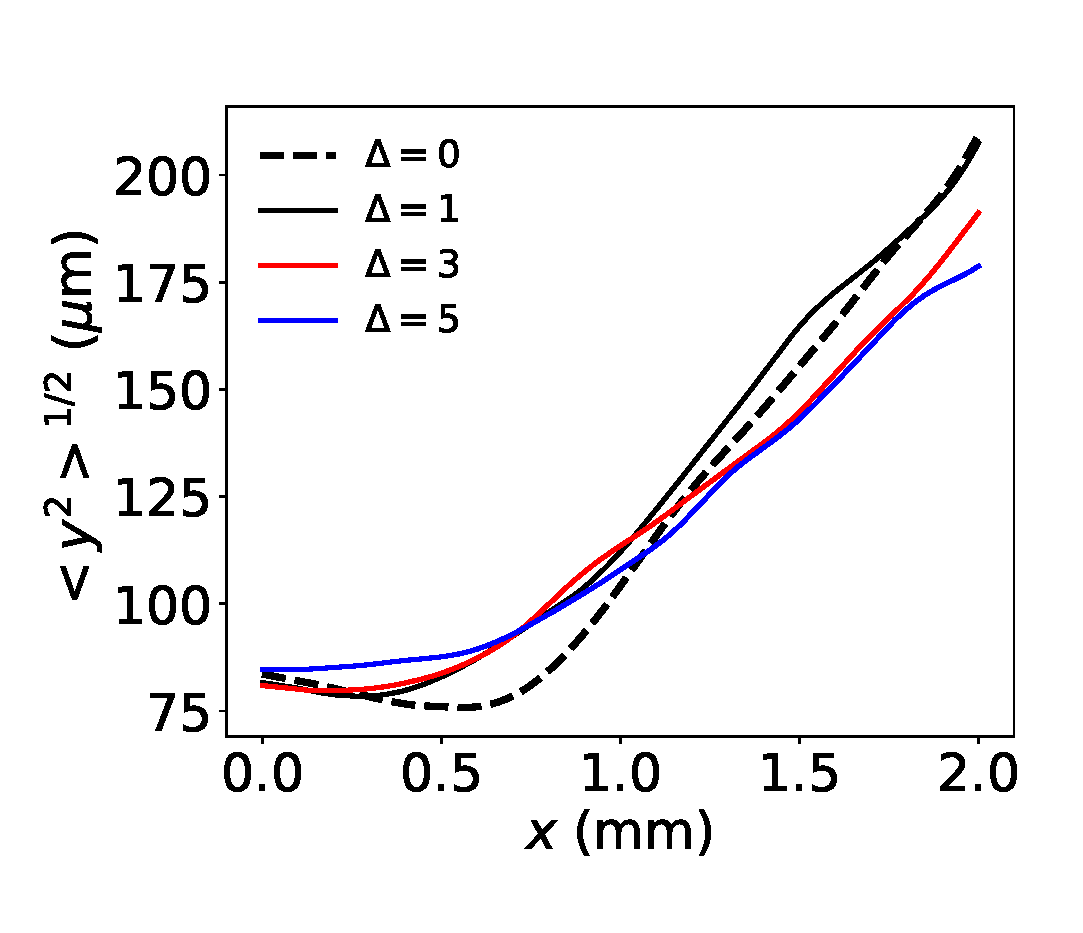
\includegraphics[width=0.35\textwidth]{FSBS_SSDL_waist_100ps.eps}
\end{tabular}
\caption{ \label{fig:ssdl} 
(a) Spatial growth rate in the $y$ direction of the forward Brillouin instability for an averaged laser intensity and wavelength $I_0=6\times 10^{14}\,\rm W/cm^2$ and  $\lambda_0=0.35\,\mu m$ and a  H$^+$  plasma with $T_e =1\,\rm  keV$, $ T_i=300\,  \rm eV$  and $n_{e}=0.1n_c$.
The RPP uses $f_\sharp = 8$ and a longitudinal  SSD [Eq. \eqref{eq:fssdl}] with  $\omega_m=2\pi \times14.25\,\rm GHz$.
(b) Transverse waist defined as $\langle y^2\rangle=\int dyI(y)y^2 /\int dyI(y)$ as a function of $x$  from the SSDL HERA   simulations at $t=100\,\rm ps$.
}
\end{figure}

\begin{figure}
\begin{tabular}{c}
(a)  $m=3$\\
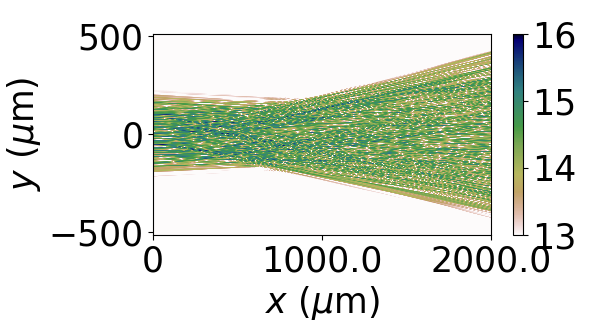
\includegraphics[width=0.4\textwidth,trim={2cm 0 0 0},clip]{ISSD1.png}\\
%(b) HERA, $m=9$\\
%\includegraphics[width=0.45\textwidth,trim={2cm 0 0 0},clip]{ISSDL3.png}\\
(b) $m=15$\\
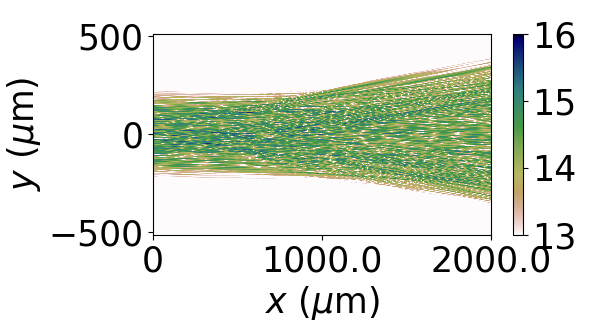
\includegraphics[width=0.4\textwidth,trim={2cm 0 0 0},clip]{ISSDL5.png}
\end{tabular}
\caption{ \label{fig:ssdl_I} 
  Intensity profile resulting from HERA  paraxial simulations  with longitudinal SSD at $t=100\,\rm ps$. The plasma and laser parameters are detailed in Fig. \ref{fig:ssdl}.
}
\end{figure}
The numerical resolution of the  longitudinal smoothing dispersion relation [Eq. \eqref{eq:fssdl}], exhibited in Fig. \ref{fig:ssdl}(a), suggests that the acoustic wave  growth remains unchanged, at least up to  $m=33$ (not shown here),  when compared to the pure RPP case (as a black dashed line). Identical results are obtained for $\xi$ in Eq. \eqref{eq:fl_ap} ranging form $1$ to $1.6$ or for  $f_L(\mathbf{k}/k_m) = \vert \mathbf{k}\vert /k_m$, which indicates that the approximation of Eq.  \eqref{eq:fl_ap} is valid  when deriving the SSDL dispersion relation.
The Hera intensity profiles obtained for different spectral dispersion strength and illustrated in Figs. \ref{fig:ssdl_I}(a,b) demonstrate that the longitudinal spectral dispersion has only a small impact on the broadening of the laser intensity profile.
Likewise the waist profiles [see Fig. \ref{fig:ssdl}(b)] present a weak  dependence of the exit plane value on $m$ which confirms our theoretical predictions and suggests that the saturation of FSBS also poorly depends on the mode number.

Note that all the paraxial simulations (either SSDT or SSDL) are compared at $t=100 \,\rm ps$,  and present similar temporal behavior: the studied asymptotic regime is longer to be reached when $m$ increases. Hence, in a realistic plasma where the hydrodynamic conditions evolves significantly with time (as for a fast-heating or a fast-expanding plasma), probably that a significant dependence of the FSBS on $m$ could be characterized in both SSDT and SSDL cases.  

\section{Polarization smoothing}
Polarization smoothing (PS) is commonly used in high energy facilities to curb laser plasma instabilities. It consists, in its idealized form, in distributing the laser energy equally over two different linear polarizations \cite[]{PRL_Moody_2001,NatPhys_Glenzer,NatPhys_Labaune}. Hence, the fields to be considered follow, in the Fourier space
\begin{equation}
    \bm E_p^\mathrm{PS} = \frac{ \Hat{\bm y}}{\sqrt{2}} E_{p,y} +  \frac{ \Hat{\bm z}}{\sqrt{2}} E_{p,z}\, ,
\end{equation}
where the two polarisation components, $E_{p,y/z}$, are given by Eq. \eqref{eq:essdwk} with independent random variables from each other [in Eq. \eqref{eq:essdwk_psi}]. Following the formalism as introduced in Secs. \ref{sec:ssdtz}, \ref{sec:ssdty} and \ref{sec:ssdl} leads to unchanged dispersion relations but with an averaged intensity, $I_0$, (or equivalently $\delta n_0/n_0$) divided by two. Hence, unlike the various spectral dispersion techniques addressed above, the impact of PS on the growth of the instabilities remains simpler to comprehend and more obvious to model. 

\section{Conclusion}
We derived the dispersion relations associated with the forward scatter of a spatially and temporally smoothed pump wave with and without polarization smoothing. Two types of SSD techniques have been  addressed, the transverse one which tends to impose a phase shift on the different frequency components in a direction transverse to the propagation axis, and the longitudinal one which results in radial phase shifts. By mean of a numerical resolution, evidence could be made that the spatial growth of the forward Brillouin scattering is weakly reduced only in the SSDT case, only in the smoothing direction and only for very large SSD strength. When looking at the growth perpendicularly to the main laser axis, or when using longitudinal SSD, no difference is found with the pure RPP case of Ref.  \cite[]{Ruyer_FSBS}. Practically, this means that the spatial growth of the pump wave aperture due to FSBS remains unaffected by the temporal  smoothing as used in existing laser facilities. Our results also confirms  that polarisation smoothing is indeed efficient in weakening the growth of the FSBS. 


Regarding the laser filamentation that could survive in the pure RPP case, we found that its growth is completely stabilize by  the use of longitudinal  temporal smoothing, even at low mode numbers. In the SSDT case, it is stabilized in the smoothing direction only.

As the effect of diffraction on the pump was ignored in our model, our predictions remain valid in the vicinity of the focal spot  for long enough focus. Moreover, more complex temporal smoothing techniques could also significantly change our conclusions.
Additionally, a  better understanding of the interplay between the FSBS and other wave mixing processes is of great importance. Indeed,  an increase of the beam aperture could also affect the properties of a Raman/Brillouin backscattering, maybe leading  to its  deflection  off the diagnostic path. 

Furthermore, we note that our dispersion relations enable the optimisation of the SSD parameters for improving the laser propagation performances and suggest that, compared to the beam properties in vacuum,  a variation of the f-cone angle is to be expected  potentially greatly  affecting the beam energy deposition region. 
Maybe more importantly, the formalism  developed here and in Ref. \cite[]{Ruyer_FSBS}  may be used to address the impact of SSD on the stimulated   Backward Brillouin instability  \cite[]{POP_Duluc_2019}, cross beam energy transfer \cite[]{PRL_Neuville_2016cbet} or Brillouin collective effects \cite[]{PRL_Neuville_2016}. 
Additionally, combining our dispersion relations with   a ray tracing scheme \cite[]{Strozzi_2017,POP_Debayle_2019} could improve the prediction capability of the vastly used radiative hydrodynamic codes for interpreting and predicting   high energy density experiments.

\section*{Acknowledgements}
We acknowledge important discussions with A. Fusaro. and G. Riazulo. 
We  admit the role of the lockdown following the COVID19 plague for forcing us to take the time to finalize this theoretical work. This work has been done under the auspices of CEA-DAM. 
% and the simulations were performed using HPC resources at TGCC/CCRT and CEA-DAM/TERA.

\section*{Data availability}
The data that support the findings of this study are available from the corresponding authors upon reasonable request.

\bibliography{biblio}
\end{document}
